\section{Engine}
\label{sec:engine}

The build pipeline engine basically wraps a common interface around the static site generator. Together with already mentioned supporting modules, it forms a nearly standalone ecosystem within a service, which happens to expose a REST API.

Other than pure HTTP services, the build engine not only has to cope with database queries -- its main purpose is to handle file input/output management based on various configurations, ideally asynchronous and possibily even in parallel. Especially the latter may cause trouble at some point, because of JavaScript's single threaded model. Though Node.js may handle asynchronous operations well, it requires its event loop to continue running, when non-blocking operations (like input/output) are executed concurrently. This differs heavily from other programming languages, which are likely to create additional threads for such kind of tasks \cite{NodejsBlockingNonblocking}.

\subsection{Asynchronous work}
Possibly one of the most important requirements of the project is to work with asynchronous calls, as well as processing them as performant as possible. As already explained, the API depends on a significant variety of tasks for fetching data to create an instance of the build pipeline according to a certain configuration.

Most of them are realized using the JavaScript Promise API, where on the one hand subsequently nesting callback functions are avoided and on the other hand, various \emph{then}-functions are not only getting chained to each other (``Promise chain''), but also returning a Promise themself \cite{MDNPromise}. This allows to keep an asynchronous flow in the same block -- some operations even allow handling more than one asynchronous function concurrently within a Promise construct.

As a result, all API calls to GitHub are realized using Promises -- as a matter of fact, the contained \emph{then}-functions are acting as necessary backbone, as the returned data often needs to be altered or even merged with the response of a second, concurrent request. One example would be the comparison of the existing file tree versus the affected files by the commit range.

\subsection{Child processes}
For keeping the API responsive to requests while a build process is running, it makes sense to decouple the heavy rendering task into an own process (``Child process''). The child process will balance the work load, so that the rendering will happen in its own V8-process on an additional processor core \cite[335]{cantelon2017node}, only able to communicate to the host process via emitting events on its built-in communication channel \cite{NodejsChildProcesses}. The host process will reside in its initial thread and only receive a message, if the child process emits one or exited -- therefore enough information will be distributed to keep the project's status in the database up to date.

There is a critical thing to consider though; since every child process gets equipped with an own memory and V8 instance, constantly allocating resources by spawning a large amount processes may lead to unexpected server crashes \cite{NodejsChildProcesses}. Virtual private servers (\emph{VPS}) with a significant amount of RAM, as well as up to 20 processor cores and more will handle such heavy tasks of course better than local machines with often less than 4 cores, but also have to be managed well in terms of resource usage. Every child process is likely to occupy a minimum of 10 megabytes of RAM by default -- though this amount surely increases. The final extent is based on the task it has to handle \cite{RobinsonNodeCluster}.

\subsection{Storage}
Because of the fact, that the project requires different stages of every repository to be stored for making use of caching, a significant amount of data has to be stored for quick access. To not loose track on the constantly growing extent, it possibly would be best to export them to long-lasting storage services like Amazon S3 buckets\footnote{\url{https://aws.amazon.com/de/s3/} -- Amazon's S3 cloud storage service.} -- however, due to the many locally hosted services (first and foremost the REST API), the decision was made in favor of also storing repository data locally in the mean time during development.

The first kind of data to outsource would surely be the rendered archive, containing the webroot. As this needs to be accessed at all time, a downtime is simply not acceptable and a constant uptime cannot be guaranteed on a service like this, unless it is also run on multiple failsafe instances around the globe.

\subsection{Realization}
After the necessary technologies for providing a non-blocking event flow were defined, the build pipeline module set could be brought in shape. Together with the wrapping REST API and the predefined endpoints (see ch. \ref{sec:structure-buildpipeline} on p. \pageref{sec:structure-buildpipeline}f), the main entry point should be able to carry the heavy load of instantiating the static site generator, as well as fetching data from GitHub. Furthermore, it should act as control interface for managing the internal communication between Metalsmith and the API.

%% Graphic of the finished workflow of the build pipeline
\begin{figure} % h-ere, t-op, b-ottom, p-age
    \centering
    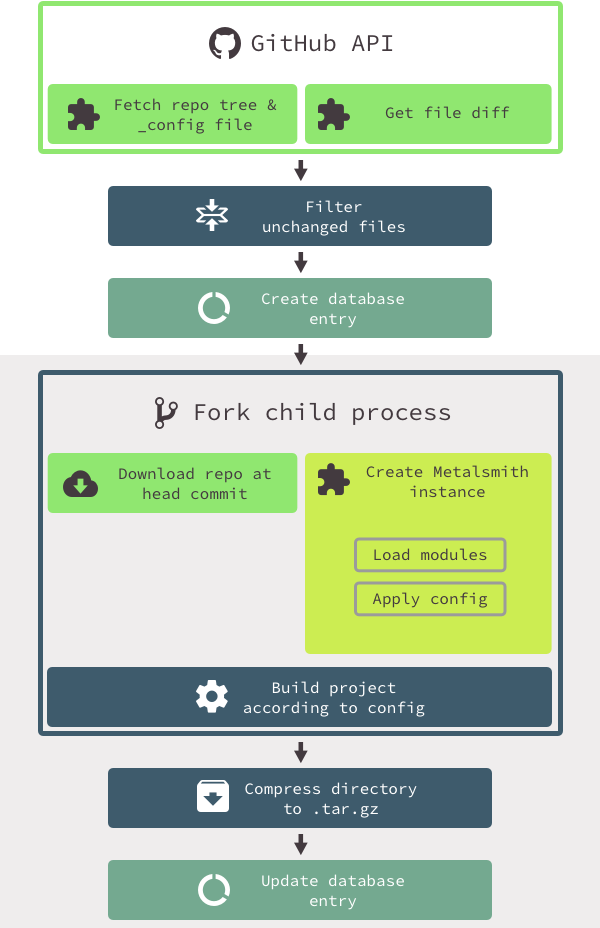
\includegraphics[width=0.75\textwidth]{application_flow.png}
    \caption{A graphic showing the main application flow of the build pipeline from top to bottom. At first, the \emph{repo tree} and \emph{file diff} are fetched from the GitHub API in parallel. After file filtering and creating a database entry, a child process is forked, which cares for executing the heavy tasks for building. After a successful build, the resulting files are compressed into a \emph{tar.gz} archive, then the database entry is updated accordingly. Afterwards, the child process is terminating gracefully.}
    \label{fig:application-flow}
\end{figure}
%

As seen in fig. \ref{fig:application-flow}, much of the build pipeline's workflow actually happens without the user knowing about (grayish area). Basically the only thing happening before sending an HTTP response, is the parsing of the configuration file, as well as filtering files, affected by the commit range. If both succeeds, the database entry is created and the user may then query the API for getting to know the current status, while the main task possibly is still running in a forked child process. So, the REST API stays responsive the whole time during build, without causing any lack of performance.

\subsubsection{Forking a child process}
According to the Node.js documentation, the \texttt{child\_process.fork()}-function is used specifically to spawn new Node.js processes. This means, that every child process creation happens without breaking the event loop of the parent process \cite{NodejsChildProcesses}. Therefore, this step is crucial before invoking any heavy task, which may result in blocking the API's responsiveness to handle additional HTTP requests.

Since the sub process is completely decoupled from the main task, it likely will not do its job in the same current working directory as its parent process. Whenever that happens, a \emph{cwd} option may be set in the configuration object upon fork \cite{NodejsChildProcesses}. The Metalsmith instance requires this feature, as every repository it will be working on is nested in a certain sub folder in the project's file tree. Most of the Metalsmith plugins are moreover designed to only work in the actual CWD, unlike its API initially proposed (see line 5 in Listing \ref{list:metalsmith} on p. \pageref{list:metalsmith}) \cite{MetalsmithRepository}.

However, equipping the child process with a cwd option was not possible at this point, as the child process also was responsible to install missing node modules. These would have been stored at the repository level -- thus, they got deleted in a subsequent build cycle, as the repository folder gets cleared prior to every download action. By omitting the cwd flag, the node modules are getting installed at the level of the REST API to make them also accessible for other website projects. Finally, the CWD gets set to the building directory via \texttt{process.chdir()} after the Metalsmith instance was configured, but before the build function was triggered.

What is additionally happening in the child task, is the following; the respective repository archive is being fetched from the GitHub API -- this happens in parallel to setting up the build pipeline:

\begin{enumerate}
  \item Creating a Metalsmith instance by setting the global API options according to the global configuration object, provided by the parent process.
  \item Filter required Metalsmith module names from the configuration object
  \item Sequentially invoke the modules to the Metalsmith instance
  \begin{enumerate}
    \item Check if the current module is already available in the main project's node modules folder,
    \item append it by default,
    \item or catch any error by appending the module name into an array of yet missing node modules.
    \item \texttt{npm install} the missing modules and repeat.
  \end{enumerate}
  \item Return the completed Metalsmith instance to the child process.
\end{enumerate}

Everything that is still missing, is waiting until both tasks (archive fetching, build pipeline setup) have succeeded, before the \texttt{build()}-function is ready to be triggered and the rendering process will be initiated. No matter if it fails or succeeds, the parent process receives a message containing necessary build information in any case.

\subsubsection{Finishing the task}
When the build pipeline was fully executed and nothing is left to do in the external JavaScript file, the process should normally exit automatically. This can be determined by listening to the \emph{close} or \emph{exit} events -- moreover, it is also possible to \emph{kill} it right from the parent process using \texttt{child.kill()} \cite{NodejsKillProcess}.

After the build pipeline finished, the CWD gets reset to its initial value, before the file tree of the rendered website is compressed into a tar.gz archive. This currently overwrites any previous archive of the same commit data -- nevertheless, any previous version may be held available by appending the respective commit hash to the file name. From this point on, any future HTTP requests trying to fetch the website archive will get provided the latest version.

To conclude the build task, the database entry finally gets updated with information about the outcome of the rendering cycle.
